\documentclass[11pt,a4paper]{article}
\usepackage[hyperref]{acl2021}
\usepackage{times}
\usepackage{latexsym}
\usepackage{graphicx}
\usepackage{caption}
\usepackage{subcaption}
\usepackage{booktabs}
\usepackage{multicol}

% \usepackage{layouts}

\graphicspath{ {./img/} }
\renewcommand{\UrlFont}{\ttfamily\small}

% This is not strictly necessary, and may be commented out,
% but it will improve the layout of the manuscript,
% and will typically save some space.
\usepackage{microtype}

\aclfinalcopy % Uncomment this line for the final submission
%\def\aclpaperid{***} %  Enter the acl Paper ID here

%\setlength\titlebox{5cm}
% You can expand the titlebox if you need extra space
% to show all the authors. Please do not make the titlebox
% smaller than 5cm (the original size); we will check this
% in the camera-ready version and ask you to change it back.

\newcommand{\nf}{\normalfont}

\title{Joint Encoding of Linguistic Information in BERT-based Language Models}

\author{%
  Apostolos Panagiotopoulos {\nf (\#14021900),} Konstantinos Papakostas {\nf (\#13914332),}\\
  {\bf Matteo Rosati} (\#13858149), {\bf Giulio Starace} (\#13010840)\\[0.25cm]
%   University of Amsterdam, Netherlands \\
  \{ \texttt{apostolos.panagiotopoulos}, \texttt{konstantinos.papakostas},\\ \texttt{matteo.rosati}, \texttt{giulio.starace} \} \texttt{@student.uva.nl}
}

\date{}

\begin{document}
\maketitle
\begin{abstract}
BERT-based Language Models (BLMs) have gained considerable popularity due to their impressive results across diverse NLP tasks. However, their representations are still not interpretable. In this work, we study the information-sharing mechanisms in BLMs and highlight the presence of joint encoding across linguistic entities, such as part-of-speech tags and dependency labels. Furthermore, we find that the way this information is shared resembles the linguistic relations between entities and is consistent across languages. Our results are validated with RoBERTa and XLM-R in English, Italian, and Greek, and take a step toward a deeper understanding of information flow in BLMs. Our code is available at \url{https://github.com/thesofakillers/bert-infoshare}
\end{abstract}

\section{Introduction}
\label{section:intro}
% ~1 page; 1 point
% Describe the problem, your research questions and goals, a summary of your findings and contributions. Please cite related work (models, datasets) as part of your introduction:
% - Introduce the task and the main goal
% - Clear research question
% - Motivating the importance of the question and explaining the expectations
% - How are these addressed or not addressed in the literature
% - What is your approach and its novelty
% - Short summary of your findings (Did you get the results you were expecting, what should one learn from your experiments and results?)

% TODO: Introduce & motivate the task we tackle as well as our main goal.

In recent years, contextualized word embeddings obtained from Large Language Models (LLMs) have consistently demonstrated state-of-the-art performance across multiple NLP tasks~\citep{devlin_bert_2019, liu_roberta_2019, wu_are_2020}. However, these representations have proven hard to interpret with regard to the information they contain, leading to a series of works~\citep{tenney_what_2018, hewitt_structural_2019, ravishankar_multilingual_2019, libovicky_language_2020, choenni_investigating_2022} that probe these models to extract insights. \citet{choenni_investigating_2022} showed that multilingual LLMs jointly encode information across languages, which inspired us to investigate whether they also jointly encode information across different linguistic entities, such as \textit{nouns} and \textit{verbs}.

% TODO: Pose clear research questions (+ expectations) & show their importance for the original task
We approach this problem by studying how two state-of-the-art models, RoBERTa~\citep{liu_roberta_2019} and XLM-R~\citep{conneau_unsupervised_2020}, encode information about part-of-speech (POS) tags and dependency relations, as well as how this information may be shared between classes. We hypothesize that these BERT-based Language Models (BLMs) learn to jointly encode words from related classes in a way that mirrors linguistic relationships. We expect to see that learned representations for linguistic features are not completely independent, with information sharing between them increasing with higher co-occurrences or functional dependencies (e.g. nouns and determinants or nominal subject and clausal subject dependencies). These overlapping relationships can vary across languages, though we anticipate that lexical entities, i.e., certain parts-of-speech such as nouns, share some degree of information in a language-agnostic manner.

% How are these addressed or not addressed in the literature & what is our approach
Our methodology leverages a cross-neutralizing method based on centroid estimation~\citep{libovicky_language_2020}, akin to the multilingual approach in \citet{choenni_investigating_2022}. In particular, we use a pre-trained instance of RoBERTa~\citep{liu_roberta_2019} as the encoder architecture and probe various layers to perform the POS tagging and dependency labeling tasks. Then, we apply the cross-neutralizing method to uncover which entities share information. We extend our experiments to the multilingual setting using XLM-R~\citep{conneau_unsupervised_2020} for the English, Greek, and Italian languages.

This work bridges the gap between analyses of multilingual information sharing and attempts to localize granular semantic and syntactic information within LLMs. ~\citet{tenney_bert_2019} and~\citet{clark_what_2019} have evaluated \textit{where} information is encoded by probing different layers within BERT. However, their work lacked an analysis of \textit{how} this information is shared. On the other hand, papers that have explored a direction similar to ours focus on how information is shared \textit{across languages}~\citep{choenni_investigating_2022}, rather than \textit{across linguistic features}. By combining these two approaches we can arrive at a more comprehensive understanding of how information about linguistic units is represented in BLMs. 

We find that similarly to typological properties of languages~\citep{choenni_investigating_2022}, information is shared across different linguistic features in BLMs. We report that this phenomenon extends to the multilingual setting in the languages tested, with variations in which labels are jointly encoded that are language-specific. Additionally, cross-lingual self-neutralization (i.e., a \texttt{NOUN} centroid from Italian used to cross-neutralize the \texttt{NOUN} class in Greek) also yields a decrease in performance, suggesting that centroids can encapsulate language-agnostic features.

\section{Related Work}
% ~ 1 page; 1 point
% Describe the existing research related to your research problem / question. Include a brief summary of the proposed methods and the key findings of the previous research.

Prior work has focused on two main approaches to inspect the data contained in contextualized embeddings; through descriptive ``probing tasks''~\citep{conneau_what_2018} and through informative subspace representations that are used to decompose word vectors~\cite{libovicky_language_2020}.

At the sentence embedding level, a prominent curated suite of probing tasks was introduced by \citet{conneau_what_2018}. These tasks examine whether sentence embeddings encode properties such as sentence length, tree depth, etc. This work is extended by \citet{hewitt_structural_2019} by proposing methods to discover linear transformations that encode word distance and tree depth in sentence parse trees using word representations. \citet{tenney_what_2018} goes further with ``edge probing'' tasks, which probe the token-level representations directly and expand to a broader range of syntactic and semantic tasks at the sub-sentence level. 

In later work, \citet{tenney_bert_2019} apply these probing methods to BERT's hidden states to quantify where linguistic information is captured within the network. They find that the model represents the steps of the traditional NLP pipeline, with lower-level, syntactic features appearing earlier than more complex semantic roles and structure. This work has been extended in the multilingual setting to probe for the previously mentioned linguistic information~\citep{ravishankar_multilingual_2019} or novel information, such as determining where typological properties of certain languages are encoded~\citep{choenni_what_2020}. Additionally, \citet{clark_what_2019} explore BERT's attention mechanism to identify what linguistic characteristics it attends to, showing that they correspond to linguistic notions of syntax and co-reference.

Other than identifying which information is encoded in word embeddings and hidden states, substantial effort has been put into trying to identify how this encoded information is shared across linguistic categories and across languages~\citep{sahin_linspector_2020, blevins_deep_2018}, with most of the work being focused on the multilingual setting~\citep{chi_finding_2020}. In particular, \citet{libovicky_language_2020} developed a method that successfully removes language-specific features without affecting encoded language-agnostic information (i.e., semantic meaning) by leveraging what they refer to as ``language centroids''. Our work draws inspiration from that of \citet{choenni_investigating_2022}, who probe for joint encoding of typological features of different languages by extending the previous method. They find that these feature values are encoded jointly across languages and are localizable in their respective language centroids.

Compared to this existing work, we apply the cross-neutralizing method to probe BLM's hidden representations for joint encoding of syntactic classes instead of languages. In sum, we apply the multilingual methods to a multi-label paradigm. Using the centroid method introduced by \citet{libovicky_language_2020} and extended in \citet{choenni_investigating_2022}, we explore what class information is independent and what is jointly encoded, as well as where in the model this information emerges. We also explore how these results vary from mono-lingual to multi-lingual models, as well as across languages.

\section{Methods}
\label{sec:methods}
% 1-2 pages; 2 points
% Cover the main techniques (“building blocks”) used in your project and intuitions behind them. Be accurate and concise.
% - How each technique that you use works (don’t just copy the formulas)
% - The relation between the techniques
% - The architecture of the final models (what layers you have, how do you do the task? how you encode the input and output? What is your loss function? Here you should provide enough information so someone could implement your models.)

\subsection{Extracting Word Representations}
\label{extracting-word-representations}
We use the base versions of RoBERTa~\citep{liu_roberta_2019} and XLM-R~\citep{conneau_unsupervised_2020} as our encoders, which produce a contextualized embedding for each sub-word token that is generated by their tokenizers. To extract a set of representations on the word level, we need to aggregate the sub-word token representations. We do so by either \textbf{(i)} taking the representation of the first sub-word token, \textbf{(ii)} taking the max-pooling over the sub-word tokens along the 768 dimensions, or \textbf{(iii)} taking the mean of the sub-word tokens.

\subsection{NLP Tasks}
\label{nlp-tasks}
To study information sharing in the aforementioned models we probe them for two well-studied NLP tasks: POS tagging and dependency labeling. For POS tagging, we encode each sentence and probe its word-level representations from a given layer $l$ using a shallow MLP. For dependency labeling, we follow a similar scheme and extract word-level representations for the child and the head of each dependency in the sentence. We concatenate them\footnote{We tested different concatenation configurations, such as including the mean vector or the absolute difference of the pair, but found the simpler approach to perform equally well.} to form a feature vector of size $2 \times H$, where $H$ is the hidden state size of the encoder model, and feed it to a shallow MLP to predict their dependency relation. We include training details for the POS tagging and dependency labeling probes in Appendix~\ref{app:probe_training}.

\subsection{Information Sharing}
\label{sec:infoshare}
% TODO: probably needs re-writing. The goal is to state the general goal.
We examine whether BLMs encode information about certain linguistic categories, such as POS tags (nouns, adjectives, etc.) or syntactic dependency relations (nominal subjects, objects, etc.) in common subspaces of their representation space.

To achieve this, we first localize the subspace of the model that corresponds to each of these categories by obtaining their mean vector representation, similarly to \citet{libovicky_language_2020}. For \textit{POS tagging}, this corresponds to the centroid of each target POS tag $t$, which, given the word representations $\mathbf{v}$, is formally defined as:
\begin{equation}
    \mathbf{u}_{t}^{(POS)} = \frac{1}{|V_t|} \sum_{\mathbf{v} \in V_t} \mathbf{v}
\end{equation}
where $V_t$ is the set of the representations of the words in our validation set that were predicted as tag $t$ when probing the $l$-th layer of our encoder. For \textit{dependency labeling}, we slightly modify the definition of the centroid, as each prediction depends on both the representation of the head $\mathbf{h}$ and the child $\mathbf{c}$ of the dependency relation. Here, the centroid of each target dependency label $t$ is defined as:
\begin{equation}
    \mathbf{u}_{t}^{(DEP)} = \frac{1}{|P_t|} \sum_{(\mathbf{h}, \mathbf{c}) \in P_t} [\mathbf{h} ~; \mathbf{c}]
\end{equation}
where $P_t$ is the set of the (head, child) representation pairs that were predicted as dependency $t$ when probing the $l$-th layer of our encoder, and $[\mathbf{h} ~; \mathbf{c}]$ is the concatenation of the two vectors.

After obtaining the mean vector $\mathbf{u}_{t}$ for each linguistic category $t$, we investigate information sharing with the cross-neutralizing method from \citet{choenni_investigating_2022}. To cross-neutralize with $\mathbf{u}_{t}$, we encode each word in the sentence using our pre-trained encoder and subtract $\mathbf{u}_t$ from its representation. We pass the resulting representations through our probing network to obtain a new distribution over the linguistic categories and re-classify words, in case of POS tagging, or words with their heads, in case of dependency labeling.

To interpret our results, we group them in (\texttt{neutralizer}, \texttt{target}) pairs, meaning that we observe the change in classification accuracy for the class \texttt{target} when neutralized with the centroid of the class \texttt{neutralizer}. In the special case where the same linguistic class is both the target and the neutralizer, we refer to our method as \textit{self-neutralizing}, and otherwise as \textit{cross-neutralizing}. We argue that pairs of linguistic categories that result in substantial drops in performance after cross-neutralizing are jointly encoded, and hence information is shared among them.

\subsection{Layer and Aggregation Selection}
\label{sec:layer-agg-selection}
The choice of the layer $l$ from which to extract the token embeddings is not arbitrary. The same non-triviality presents itself in the choice of aggregation function mentioned in Section~\ref{extracting-word-representations}. An ideal selection should capture the greatest amount of information for the words and the task at hand. For each aggregation function, we self-neutralize using embeddings from different layers and compare the relative drop in self-neutralizing accuracy.

We hypothesize that the configurations where the self-neutralizing percentage drop is the greatest are those closest to an ideal selection, as a higher decrease in performance signals in a higher amount of information being captured in the centroids. We also consider that this drop should be relative to a high baseline accuracy, to achieve more accurate centroid definitions. Therefore, we take the top quartile of our configurations in terms of baseline accuracy, rank them in descending order of relative drop in accuracy, and select the first to perform cross-neutralization.

\section{Experiments}
% ~1/2 - 1 page; 1 point
% Describe your experimental setup. The information here should allow someone else to exactly re-create your experiments. Describe how you evaluate the models.
%% - Explain the task and the data
%% - Training the models (model, data, parameters and hyper parameters of the models, training algorithms, what supervision signals you use, etc.)
%% - Evaluation (e.g. metrics)
\subsection{Datasets}
We use the Universal Dependencies framework~\citep{nivre_universal_2020} to train our probing models in POS tagging and dependency labeling, as it offers a consistent annotation style across a collection of treebanks over multiple languages. In particular, we use the GUM corpus~\citep{zeldes_gum_2017} for English, which consists of 9,130 sentences with a total of 164,488 words, the VIT corpus~\citep{delmonte_vit_2017} for Italian with 10,087 sentences and 279,723 total words, and the GDT corpus~\citep{prokopidis_universal_2017} for Greek with 2,521 sentences and 63,441 total words.

All of the datasets contain token-level annotations with a total of 17 possible POS tags and 36 dependency relations. Additionally, for dependency relations, a unique head corresponds to each word, with the exception of the \texttt{root} relation, which has no head, and hence it is omitted. A detailed description of the pre-processing pipeline for all three treebanks can be found in Appendix~\ref{app:dataset_preprocess}.

\subsection{Baseline Models}
We use RoBERTa and XLM-R\footnotemark as our encoders, and we keep their weights frozen while training our probe classifiers on the aforementioned datasets for both tasks. We try various combinations of layers to probe ($l \in \{1, 3, 6, 9, 12\}$) and sub-word token aggregations (\texttt{first}, \texttt{mean}, \texttt{max-pooling}), and use the one that achieves a high baseline accuracy while resulting in the largest accuracy drop when self-neutralizing, as described in Section~\ref{sec:layer-agg-selection}. We display the results we obtained per configuration in Appendix~\ref{app:probe_config}. We report the classification accuracy for the best self-neutralizing combination for all our baseline models in Table~\ref{tab:baseline_acc}, and we observe that we are in line with the current literature~\citep{straka_evaluating_2019}. As we only employ a pre-trained encoder without fine-tuning on our corpus, we expect to see a slightly lower accuracy compared to state-of-the-art approaches in each task.
\footnotetext{The pre-trained models are available on Hugging Face: \url{https://huggingface.co/roberta-base}
\url{https://huggingface.co/xlm-roberta-base}}
%\footnotetext{A short analysis on how we selected the optimal configuration in each case can be found in Appendix~\ref{app:probe_config}.}

\begin{table}[ht]
\small
\centering
\begin{tabular}{c|c|ccc|}
             & \textbf{RoBERTa} & \multicolumn{3}{c|}{\textbf{XLM-R}}                    \\ \cline{2-5} 
             & \textbf{en\_gum} & \textbf{en\_gum} & \textbf{it\_vit} & \textbf{el\_gdt} \\ \cline{2-5}
\textbf{POS} & 95.6\%           & 95.5\%           & 97.4\%           & 97.9\%           \\
\textbf{DEP} & 90.9\%           & 91.4\%           & 93.9\%           & 94.8\%           
\end{tabular}
\caption{Classification accuracy for part-of-speech tagging and dependency labeling for our baseline models.}
\label{tab:baseline_acc}
\end{table}

\subsection{Cross-Neutralizing in English}
To perform cross-neutralization, we subtract the centroid of a given label (\texttt{neutralizer}) from the embeddings of our encoder and compare the accuracy drop over the labels (\texttt{targets}). Although it is reasonable to expect that subtracting a fixed vector from our embeddings might always cause a performance drop, we experimented with subtracting random vectors and noticed that the performance remained unchanged. Thus, we argue that considerable changes in accuracy for a (\texttt{neutralizer}, \texttt{target}) pair suggest that the model learns some information about these two classes jointly.

While the labels for POS tagging are trivially bound to a single word, dependency labels refer to pairs of child and head words, leading to the definition of centroids being less straightforward. We experiment with considering only the embedding of the child as the centroid, versus a concatenation of both the child and the head. The latter results in more consistent self-neutralization across the task labels, which we assume suggests a better choice for centroid definition. Therefore, we use this concatenation configuration in all further dependency labeling cross-neutralization analyses.

\subsection{Monolingual vs Multilingual Models}
We also extend our experiments to the multilingual setting using XLM-R as the encoder and evaluating cross-neutralization in three different languages. This lets us both verify the consistency of our method across models, as we can directly compare the results between RoBERTa and XLM-R in English, but also across languages, as we can compare the effects of cross-neutralization on English, Italian, and Greek. By doing so, we can also assess the effect of cross-neutralization at a language-family level, as these are three Indo-European languages.

\subsection{Cross-Lingual Cross-Neutralizing}
In the multilingual setting, we test whether our findings are consistent across languages. A different direction worth exploring is whether there is a joint encoding of information between two related linguistic categories from two different languages. We test this hypothesis by cross-neutralizing every linguistic entity in one language with another entity from another language, e.g. all Italian POS tags with English nouns. 


\subsection{Cross-Task Cross-Neutralizing}
% WIP, TODO
To study joint sharing of linguistic information \textit{across tasks}, we additionally subtract the POS centroids from the child embeddings in child-parent concatenations for dependency labelling. In this way we effectively cross-neutralise across tasks, with POS neutralizers and dependency label targets. Similarly, we subtract the child portion of the dependency label centroids from the POS embeddings for POS tagging, to test whether any sort of joint learning happens in both directions.  

\section{Results \& Analysis}
% \subsection{Self-neutralization}
% We have mentioned this in both section 3.4 (why self-neutralize to pick a model), and in section 4.2 with a pointer to appendix. Maybe we can skip this subsection in the analysis

\subsection{Monolingual Cross-Neutralization}
\label{sec:evaluation-monolingual}
The decrease in accuracy when cross-neutralizing English POS tags and dependency labels is presented in Figure \ref{fig:xneutr_roberta}. Overall, we observe a pattern that verifies our hypothesis that related classes are jointly encoded in RoBERTa, for both the POS and DEP tasks. Subtracting the centroids associated with specific classes leads to a decrease in accuracy for other classes, indicating that information is shared across them. Notably, this cross-neutralizing phenomenon is not necessarily symmetric; in several instances, the accuracy change for a label $y$ when using neutralizer $x$ is not similar in magnitude to the accuracy change for $x$ when $y$ is the neutralizer. This may be due to the structure of language, which can be represented as a directed graph in which linguistic entities may modify others, but may not themselves be modified by their object. For example, adjectives modify nouns, and yet nouns do not modify adjectives. Further work could further clarify why certain entities cross-neutralize symmetrically and why others do not. In the rest of this subsection, we kept a subset of the linguistic categories both for the POS and DEP tasks, to highlight some task-specific patterns that emerge from our cross-neutralizing experiments. The figures containing the cross-neutralizing results between all classes can be found in Appendix~\ref{app:full_xneutr}.

\begin{figure}[t]
\centering
\includegraphics[width=\columnwidth]{roberta-base_multifigure_sampled.eps}
\caption{Relative change in accuracy when cross-neutralizing 8 sampled POS (top) and DEP (bottom) tags using embeddings from RoBERTa in English.}
\label{fig:xneutr_roberta}
\end{figure}

\begin{figure*}[t]
\centering
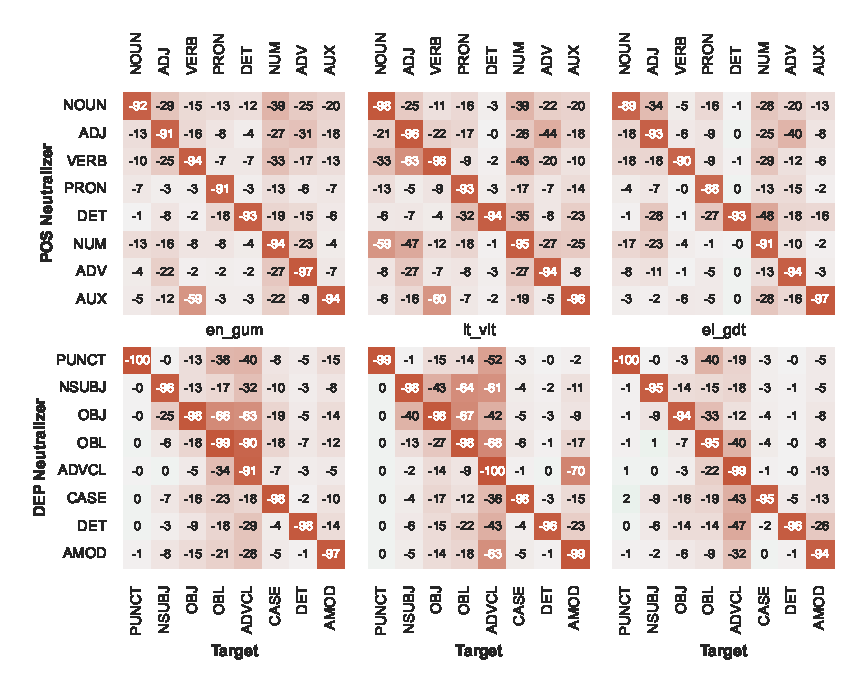
\includegraphics[width=\textwidth]{xlm_multifigure_sampled.eps}
\caption{Relative  change in accuracy when cross-neutralizing 8 sampled POS (top) and DEP (bottom) tags using embeddings from XLM-R in English (left), Italian (center) and Greek (right).}
\label{fig:xneutr_xlmr}
\end{figure*}

\paragraph{POS Tagging}
The top part of Figure~\ref{fig:xneutr_roberta} shows the impact of cross-neutralization on a selection of POS tags. The shown POS tags have been selected to ensure a fair distribution between open and closed-class words. We observe that while there is evidence of linguistically related units being jointly encoded, this phenomenon is not ubiquitous. For instance, we see that the auxiliaries (\texttt{AUX}) and verbs (\texttt{VERB}) are jointly encoded, as indicated by the relative decrease of 53\% in VERB classification accuracy. This aligns with our hypothesis since auxiliaries can be considered function words acting on verbs. However, the same is not observed when neutralizing nouns (\texttt{NOUN}) with determiner (\texttt{DET}) centroids, where the relative percentage decrease is only 2\%, suggesting that these tags are learned independently, despite determiners acting as a lexical modifier for nouns. Finally, we note how certain tags are particularly susceptible to (such as numerals, \texttt{NUM}) or adept at (such as \texttt{NOUN}) cross-neutralization, regardless of their relationship to the neutralizer or target.

\paragraph{Dependency Labeling}
The lower half of Figure~\ref{fig:xneutr_roberta} also shows the impact of cross-neutralization on a selection of dependency labels. These labels were selected to highlight the major trends in joint encoding within this task. We observe that information sharing is most pronounced when dependency classes are (\textbf{1}) closely related by definition, or (\textbf{2}) hierarchically connected. Both of these aspects support our hypothesis of joint encoding of linguistically related dependencies and elevate important details of linguistic structure. As an example of (\textbf{1}), one can consider the classes \texttt{NSUBJ}, \texttt{OBJ}, and \texttt{OBL}. Each is jointly encoded with the others, as they help define the basic syntactic structure of the sentence in relation to the predicate. 

On the other hand, the results of \texttt{PUNCT} and \texttt{ADVCL} lend support to (\textbf{2}). \texttt{ADVCL} is a clausal dependency, and is therefore significantly affected when removing information that is more related to word components of clauses such as \texttt{OBJ}, \texttt{AMOD}, \texttt{CASE}, and \texttt{PUNCT}. This latter dependency is quite noteworthy; it is a strong neutralizer across several classes, and yet is not affected by the removal of any other centroid. Punctuation plays a strong role in defining the syntactic tree of a sentence and therefore removing that information will distort its structure and thus the predicted dependency labels. For example, we can consider the striking difference between the sentences ``let's eat, grandma" and ``let's eat grandma".
On the other hand, one can read a sentence in a foreign language and still be able to point out the punctuation, indicating that, even with limited information, punctuation information is orthogonal to other linguistic features.

\subsection{Multilingual Cross-Neutralization}
\label{sec:evaluation-multilingual}
In this section, we repeat the evaluation of Section~\ref{sec:evaluation-monolingual} using embeddings from XLM-R trained on English, Italian and Greek datasets and report results in Figure~\ref{fig:xneutr_xlmr}. To facilitate comparison both across languages and with the results acquired from RoBERTa, we make the same selection of POS tags and dependency labels and present the full results in Appendix \ref{app:full_xneutr}.

\paragraph{Consistency Across Models}
When comparing RoBERTa and XLM-R on the English dataset, we observe similar patterns across linguistic categories for both POS tagging and dependency labeling. For example, numerals seem to be jointly encoded with nouns and auxiliaries. This supports the idea that even in a multilingual training setting, the linguistic entities of each language are encoded similarly to a monolingual model.

\paragraph{Consistency Across Languages}
Similar patterns can also be observed when comparing across languages in XLM-R. For instance, we see that nouns consistently neutralize numerators by a significant factor. Likewise, in the dependency labeling setting, we note that the lack of neutralization of determiners (\texttt{DET}) is consistent across all three languages. This suggests that the tags involved in the cross-neutralization pairs where this observation holds are language-agnostic. On the same note, language-specific behavior is also evident. For instance, \texttt{VERB} POS tags cross-neutralize adjectives (\texttt{ADJ}) more prominently in Italian than in the other two languages. Similarly, while the neutralization of \texttt{ADVCL} by \texttt{NSUBJ} in English dependency labeling is significant, the effect is less pronounced in the other two languages. The results suggest that XLM-R discovers and leverages language-agnostic information when possible, while also learning language-specific information when necessary.

\subsection{Cross-Lingual Cross-Neutralization}
We extend the experiments of the previous section by cross-neutralizing using linguistic categories from different languages. Figure~\ref{fig:crosslingual_xneutr_xlm} shows the results of cross-neutralizing for Italian POS tagging and dependency labeling when using the corresponding English centroids from each linguistic category. We notice a substantial drop in performance across the diagonals of these graphs, which correspond to the self-neutralizing scenario. This indicates the presence of information sharing between languages but is limited to the same linguistic feature. We also observe a correlation between different features of different languages, such as Italian adverbs and English adjectives, or Italian nominal subjects and English objects. This behavior highlights the tremendous learning capacity of these models, as information can be shared between the representations for different languages.

Finally, we repeat the experiment by using English neutralizers on the Greek corpus, and we observed similar but milder trends. We hypothesize that this is due to English being linguistically closer to Italian than Greek, which leads to a higher degree of information sharing between these two languages. For more detailed plots on cross-lingual cross-neutralization, we refer the reader to Appendix \ref{app:full_xneutr}.

\begin{figure}[t]
\centering
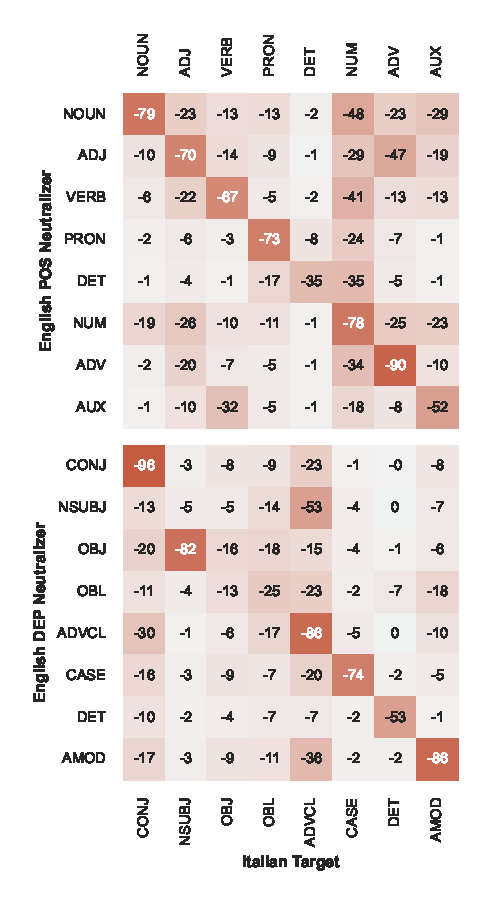
\includegraphics[width=\columnwidth]{cross-lingual_it_from_en_multifigure_sampled.eps}
\caption{Relative change in accuracy when cross-neutralizing Italian with 8 sampled POS (top) and DEP (bottom) English tags using embeddings from XLM-R.}
\label{fig:crosslingual_xneutr_xlm}
\end{figure}

\section{Conclusion}
% Conclusion (~1/4 page, 1 point). The main conclusions of your experiments.
% - What have you learned from you experiments? how does it relate to what is already known in the literature?
% - Where the results as expected? any surprising results? why?
% - Based on what you learned what would you suggest to do next?

In this work, we studied the joint encoding of linguistic entities in BLMs. We approached the problem by cross-neutralizing pairs of entities in two well-studied tasks: POS tagging and dependency labeling. We first evaluated our methodology in a simple monolingual scenario using RoBERTa and found joint encoding of similar linguistic categories for both tasks. We extended our evaluation to include XLM-R and found our hypothesis to hold both across languages and to be persistent across two different BERT-based models. Finally, we noticed that related linguistic categories are jointly encoded across different languages in XLM-R.

Our findings are consistent with recent work on information sharing in BLMs and shed light on the flow of information within them. They also give credit to the efficacy of multilingual models over the use of multiple monolingual ones. We hope that our work will aid the exploration and interpretation of BLMs and encourage further research on their information-sharing mechanisms. As a future direction, we would like to extend our experimental setting to include more downstream NLP tasks and evaluate our findings in more languages.

\bibliographystyle{acl_natbib}
\bibliography{references}

\clearpage

\appendix

\section{Training details for the probes}
\label{app:probe_training}
For both tasks, we opt for a two-layer MLP probe with a $\tanh$ activation. During training, we keep the encoder’s parameters frozen and train the linear probes using the AdamW optimizer~\citep{loshchilov_decoupled_2019} with a learning rate of $10^{-3}$ and weight decay of $10^{-2}$, and employ early stopping according to the validation set accuracy.

\section{Dataset pre-processing}
\label{app:dataset_preprocess}
The sentences in the corpora from the Universal Dependencies framework are already tokenized to the word level and stored as lists of words in the \texttt{tokens} field. However, since we use sub-word tokenizers, namely the Byte Pair Encoding~\citep{sennrich_neural_2016} and SentencePiece~\citep{kudo_sentencepiece_2018} tokenizer, we further split the words into their sub-word tokens. Depending on the task, we also include either the \texttt{upos} field, which is a list of integers corresponding to one of the 17 universal POS tags available, or the \texttt{head} and \texttt{deprel} fields which contain the head and one of the 36 dependence relations for dependency labeling\footnotemark. It should be noted that we only keep the language-independent relations, as some of them appear only with a language-specific modifier, and including them would make comparisons across languages less straightforward.
\footnotetext{A full list of \href{https://universaldependencies.org/u/pos/all.html}{POS tags} and \href{https://universaldependencies.org/u/dep/all.html}{dependency relations} can be found on the Universal Dependencies website.}

Furthermore, upon inspecting the datasets we observed that the annotators had split contractions into their parts and included them next to the original contraction for the Italian and Greek corpora. However, ground-truth labels were only provided for the sub-words, with the compound words annotated as a special class ``\_''. Hence, we filtered out the compound words from these datasets and retained their sub-parts. In addition to that, for dependency labeling, we ignored words with the root dependency label, as they have no head and their prediction is trivial.

\section{Choosing a configuration for probing}
\label{app:probe_config}
Figures \ref{fig:selection_roberta} and \ref{fig:selection_xlm} showcase the decrease in accuracy when self-neutralizing in the POS tagging/dependency labeling task for RoBERTa and XLM-R accordingly. We report the best configurations for each model, language, and task combination in Table~\ref{tab:configurations}, and correspond to the ones we used for our cross-neutralization experiments.

\begin{table*}[ht]
\centering
\begin{tabular}{@{}lccccc@{}}
\toprule
 & \multicolumn{2}{c}{\textbf{POS}} & \multicolumn{3}{c}{\textbf{DEP}} \\ \midrule
\textbf{Encoder / treebank} & \textbf{Layer} & \textbf{WP Aggregation} & \textbf{Layer} & \textbf{WP Aggregation} & \textbf{Concatenation} \\
RoBERTa / en\_gum & 3 & max & 3 & mean & {[}child ; head{]} \\
XLM-R / en\_gum & 9 & max & 9 & first & {[}child ; head{]} \\
XLM-R / it\_vit & 9 & first & 9 & mean & {[}child ; head{]} \\
XLM-R / el\_gdt & 12 & mean & 9 & mean & {[}child ; head{]} \\ \bottomrule
\end{tabular}
\caption{The best probing configuration for each encoder model (RoBERTa \& XLM-R), task (POS \& DEP) and language (English, Italian \& Greek) combination, chosen as outlined in Section~\ref{sec:layer-agg-selection}. Ultimately, these are the configurations that we use for all of our cross-neutralization experiments.}
\label{tab:configurations}
\end{table*}

\begin{figure}[ht]
    \centering
    \begin{subfigure}{\columnwidth}
        \centering
        \includegraphics[width=\textwidth]{configs/roberta-base_config_selection_POS.pdf}
        \caption{Accuracy decrease for \textbf{POS tagging} when using different WordPiece aggregations.}
        \label{fig:pos_selection_roberta}
    \end{subfigure}
    \begin{subfigure}{\columnwidth}
        \centering
        \includegraphics[width=\textwidth]{configs/roberta-base_config_selection_DEP.pdf}
        \caption{Accuracy decrease for \textbf{dependency labeling} when using different WordPiece aggregations and child-head concatenation configurations.}
        \label{fig:dep_selection_roberta}
    \end{subfigure}
    \caption{Decrease in performance for RoBERTa when \textbf{self-neutralizing} in the POS tagging (top) and dependency labeling (bottom) tasks using embeddings extracted from different layers and setup configurations.}
    \label{fig:selection_roberta}
\end{figure}

\begin{figure*}[ht]
    \centering
    \begin{subfigure}{\columnwidth}
        \centering
        \includegraphics[width=.9\textwidth]{configs/xlm-roberta-base_config_selection_POS.pdf}
        \caption{POS tagging Accuracy Decrease using different WordPiece
aggregations.}
        \label{fig:pos_selection_xlm}
    \end{subfigure}
    \begin{subfigure}{\columnwidth}
        \centering
        \includegraphics[width=.9\textwidth]{configs/xlm-roberta-base_config_selection_DEP.pdf}
        \caption{Dependency labeling Accuracy Decrease using different WordPiece aggregations.}
        \label{fig:dep_selection_xlm}
    \end{subfigure}
    \caption{Decrease in performance for XLM-R when \textbf{self-neutralizing} in the POS tagging (left) and dependency labeling (right) tasks using embeddings extracted from different layers and setup configurations, for each of for English (en\_gum), Italian (it\_vit) and Greek (el\_gdt) treebanks. For dependency labeling, we use the best child-head concatenation mode (ONLY) based on the results we aquired with RoBERTa, as shown in Figure~\ref{fig:dep_selection_roberta}.}
    \label{fig:selection_xlm}
\end{figure*}

Figure~\ref{fig:xneutr_childonly} shows the results of cross-neutralizing in the dependency labeling task when the centroids are based exclusively on the child word's representation. As mentioned in Section~\ref{sec:evaluation-monolingual}, this results in less prominent self-neutralizing. We hypothesize that the inclusion of information about the head within the centroid is likely leveraged by the classifier to retain good accuracy.

\begin{figure*}[p]
    \centering
    \includegraphics[width=\textwidth]{full_figures/DEP_child_only_roberta-base_en_gum_acc_drop_agg=mean_probe=3.eps}
    \caption{Relative change in accuracy when cross-neutralizing DEP tags using embeddings from RoBERTa on en\_gum, in a setup configuration where we \textbf{only use the child embeddings} for the centroid calculation.}
    \label{fig:xneutr_childonly}
\end{figure*}

\section{Detailed cross-neutralizing results}
\label{app:full_xneutr}
We display the complete results for our cross-neutralization experiments in Figures \ref{fig:xneutr_roberta_pos_complete} -- \ref{fig:xlingual_xneutr_dep_en_gum_from_el_gdt}. More specifically, Figures \ref{fig:xneutr_roberta_pos_complete} and  
\ref{fig:xneutr_roberta_dep_complete} correspond to the monolingual setting with RoBERTa on English, Figures \ref{fig:xneutr_xlm_pos_en_complete} -- \ref{fig:xneutr_xlm_dep_gr_complete} to the multilingual with XLM-R on English, Italian and Greek. Figures \ref{fig:xlingual_xneutr_pos_el_gdt_from_en_gum} -- \ref{fig:xlingual_xneutr_dep_en_gum_from_el_gdt} show the cross-lingual setting for every possible pairing of our three languages with XLM-R.

% POS roberta
\begin{figure*}[t]
    \centering
    \includegraphics{full_figures/POS_xlm-roberta-base_en_gum_acc_drop_agg=max_probe=9.eps}
    \caption{Relative change in accuracy when cross-neutralizing POS tags using RoBERTa embeddings on en\_gum.}
    \label{fig:xneutr_roberta_pos_complete}
\end{figure*}

% DEP roberta
\begin{figure*}[t]
    \centering
    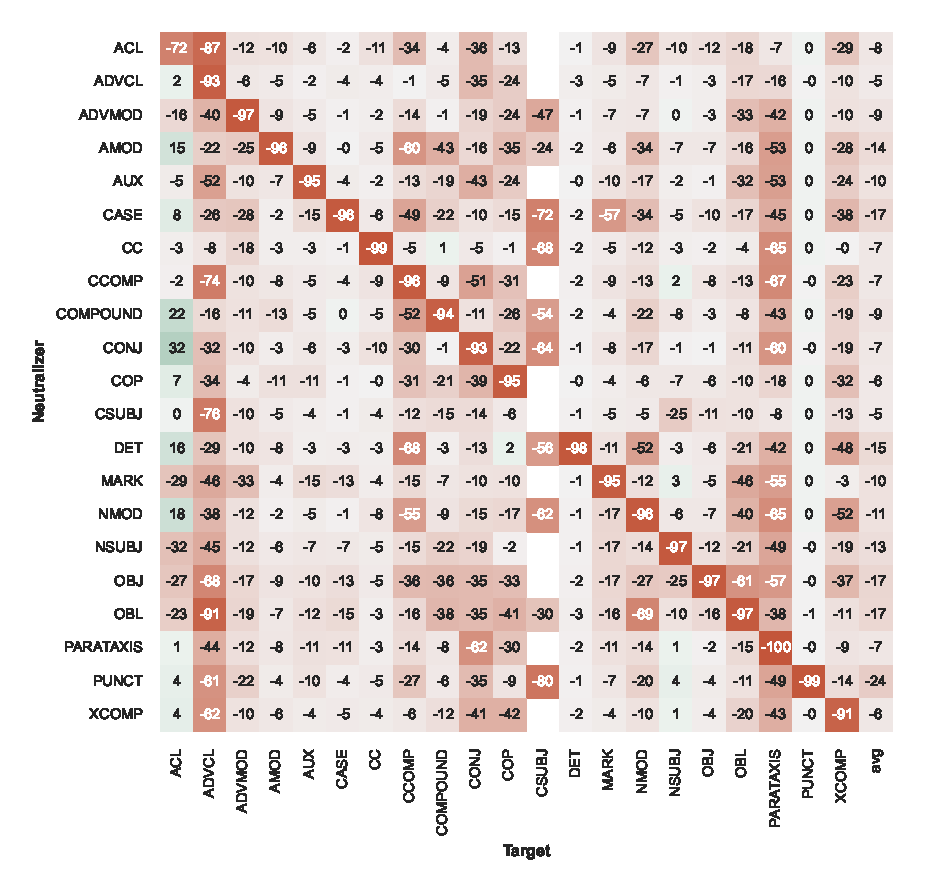
\includegraphics{full_figures/DEP_roberta-base_en_gum_acc_drop_agg=mean_probe=3_concat-mode=ONLY.eps}
    \caption{Relative change in accuracy when cross-neutralizing DEP tags using RoBERTa embeddings on en\_gum. Note the relative increase in performance for the \texttt{PARATAXIS} relation; this is likely due to noise, as \texttt{PARATAXIS} labels make up less than $1\%$ of the dataset.}
    \label{fig:xneutr_roberta_dep_complete}
\end{figure*}

% POS tags XLM en, it, gr
\begin{figure*}[t]
    \centering
    \includegraphics{full_figures/POS_xlm-roberta-base_en_gum_acc_drop_agg=max_probe=9.eps}
    \caption{Relative change in accuracy when cross-neutralizing POS tags using XLM-R embeddings on en\_gum.}
    \label{fig:xneutr_xlm_pos_en_complete}
\end{figure*}

\begin{figure*}[t]
    \centering
    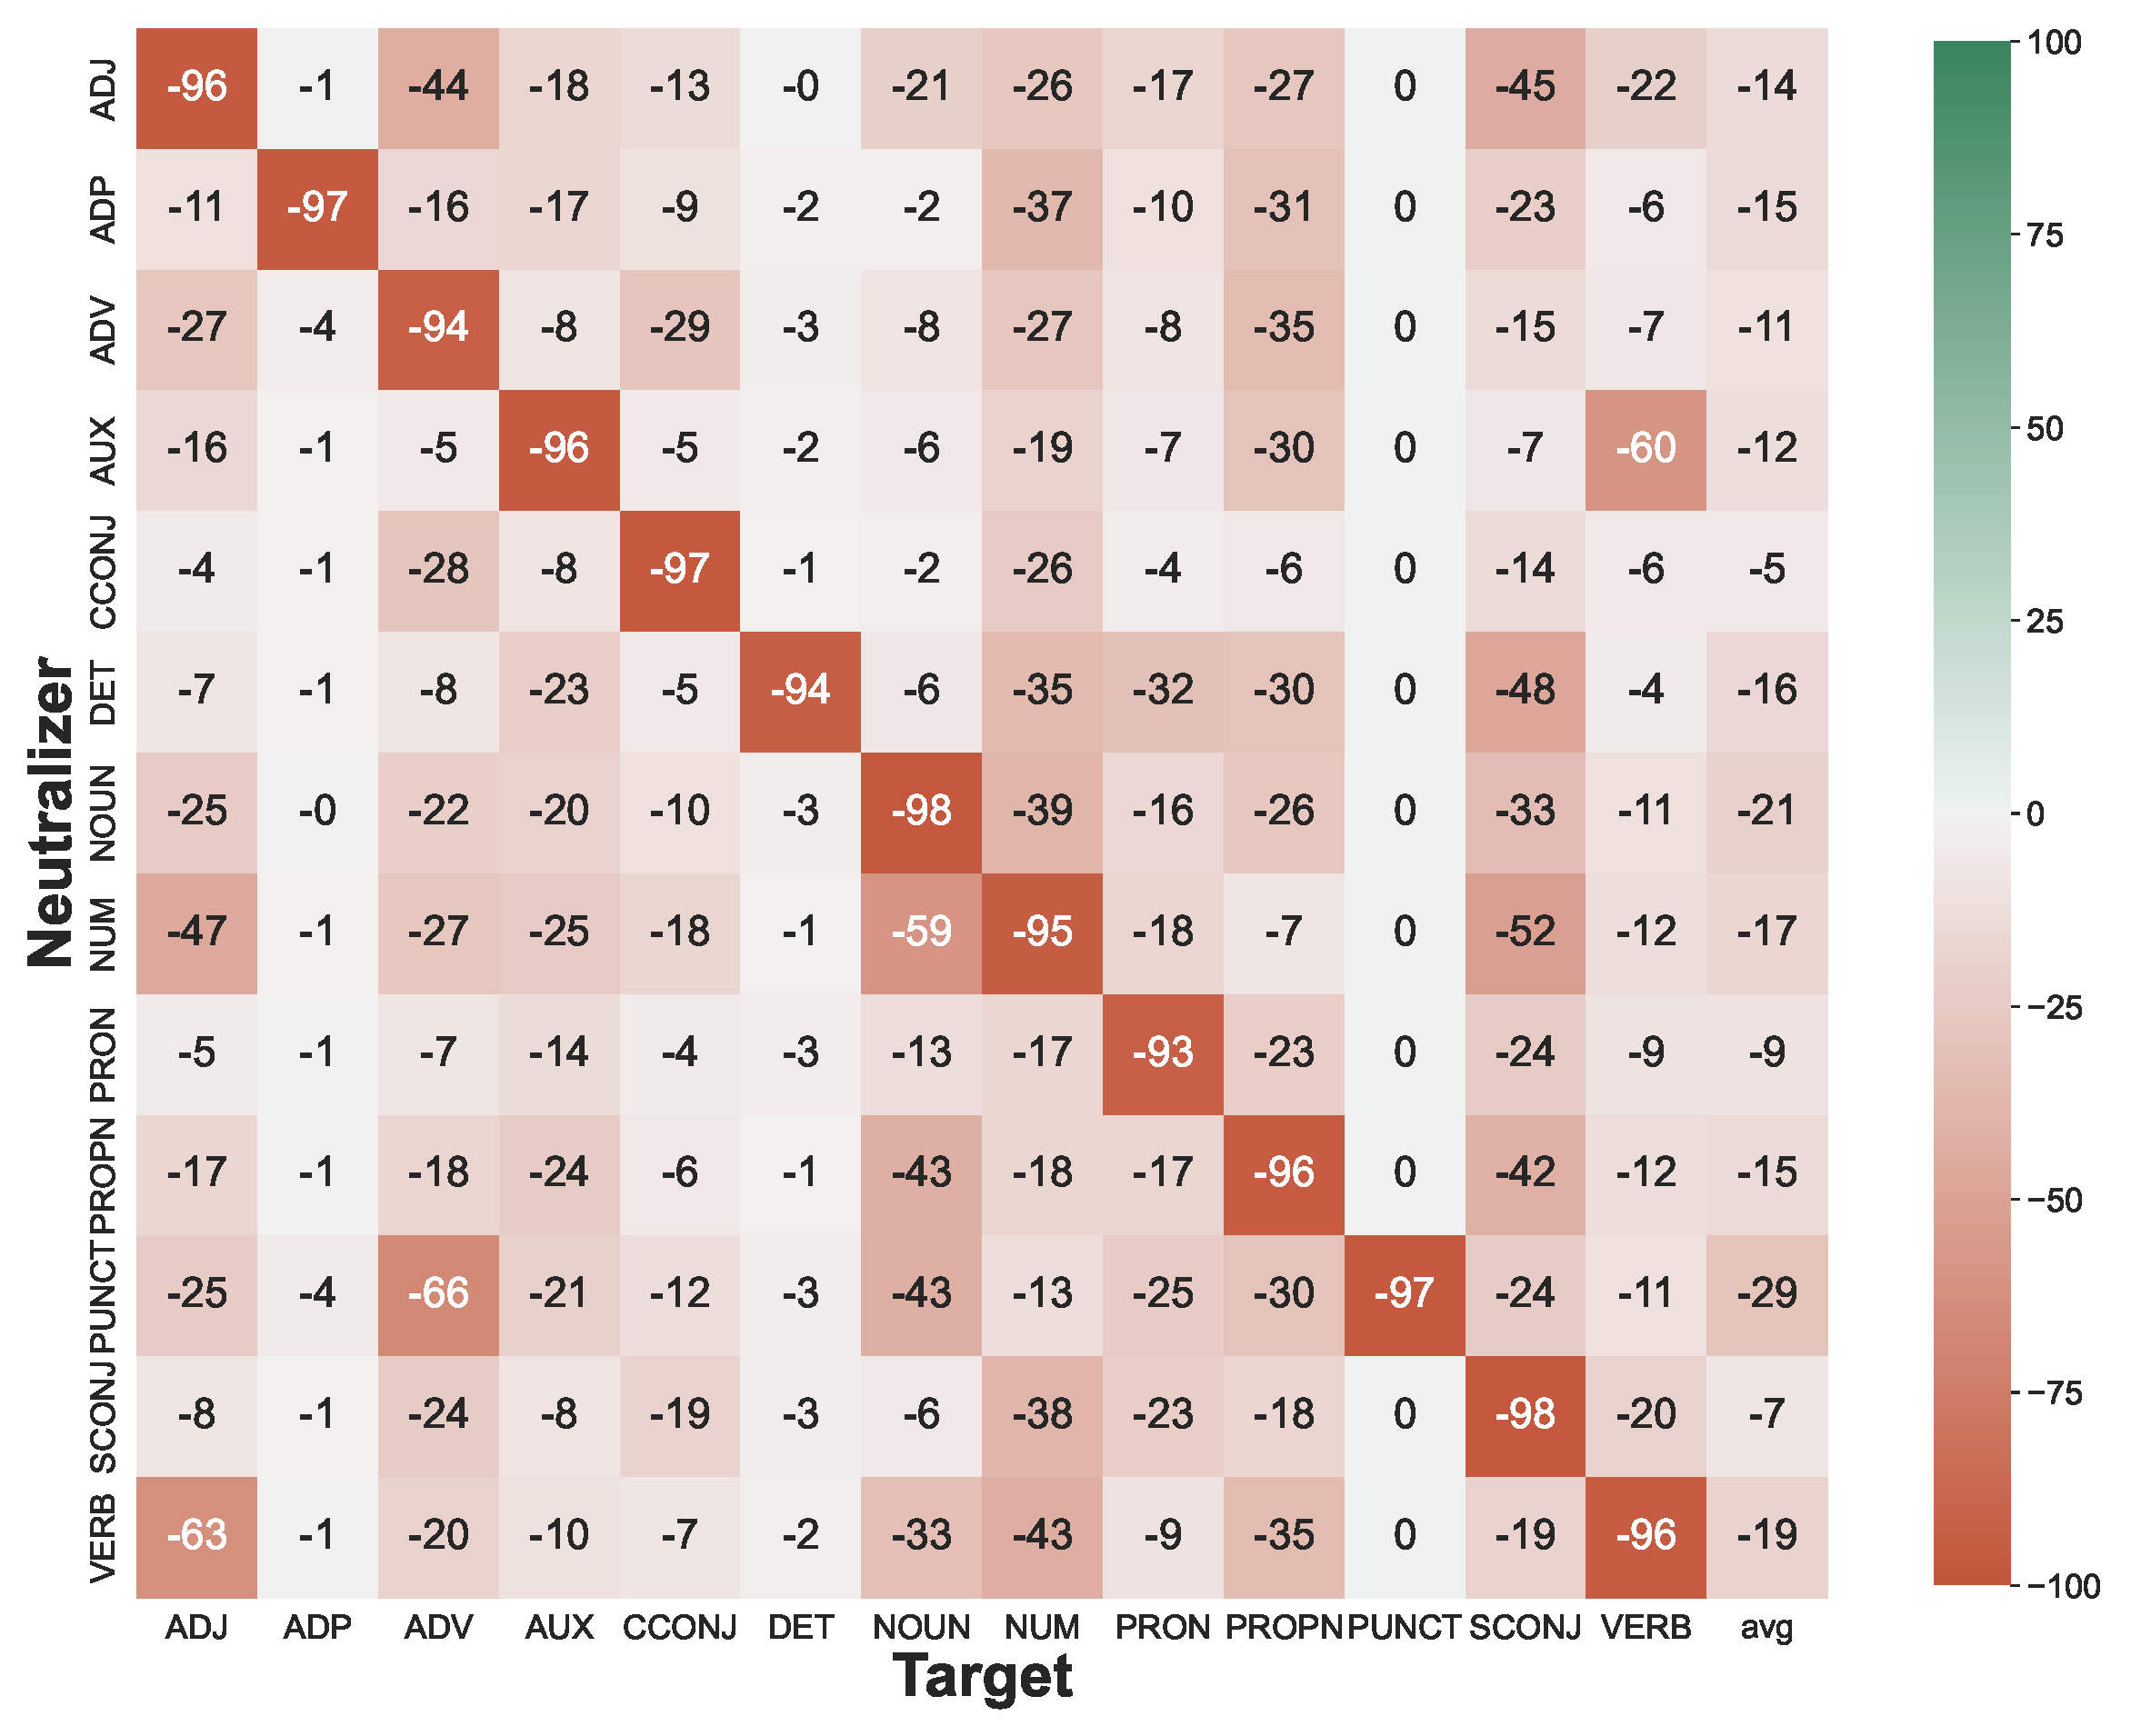
\includegraphics{full_figures/POS_xlm-roberta-base_it_vit_acc_drop_agg=first_probe=9.eps}
    \caption{Relative change in accuracy when cross-neutralizing POS tags using XLM-R embeddings on it\_vit.}
    \label{fig:xneutr_xlm_pos_it_complete}
\end{figure*}

\begin{figure*}[t]
    \centering
    \includegraphics{full_figures/POS_xlm-roberta-base_el_gdt_acc_drop_agg=mean_probe=12.eps}
    \caption{Relative change in accuracy when cross-neutralizing POS tags using XLM-R embeddings on el\_gdt.}
    \label{fig:xneutr_xlm_pos_gr_complete}
\end{figure*}

% DEP tags XLM en, it, gr
\begin{figure*}[t]
    \centering
    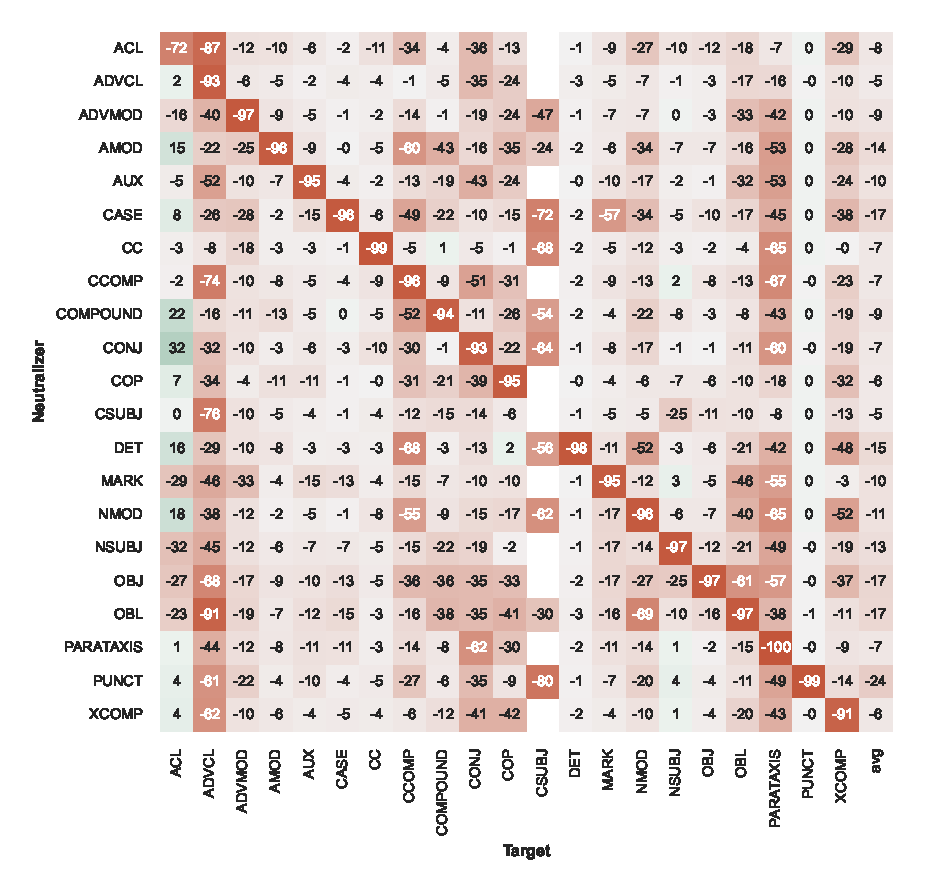
\includegraphics{full_figures/DEP_roberta-base_en_gum_acc_drop_agg=mean_probe=3_concat-mode=ONLY.eps}
    \caption{Relative change in accuracy when cross-neutralizing DEP tags using XLM-R embeddings on en\_gum.}
    \label{fig:xneutr_xlm_dep_en_complete}
\end{figure*}

\begin{figure*}[t]
    \centering
    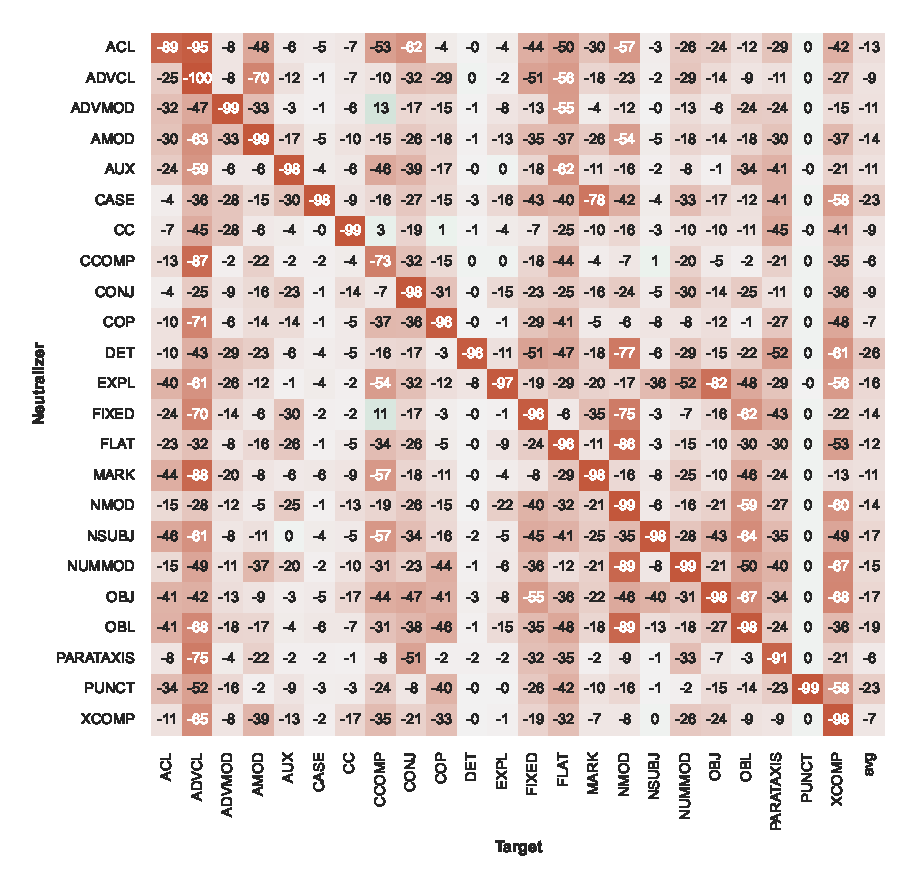
\includegraphics{full_figures/DEP_xlm-roberta-base_it_vit_acc_drop_agg=mean_probe=9_concat-mode=ONLY.eps}
    \caption{Relative change in accuracy when cross-neutralizing DEP tags using embeddings from XLM-R on it\_vit.}
    \label{fig:xneutr_xlm_dep_it_complete}
\end{figure*}

\begin{figure*}[t]
    \centering
    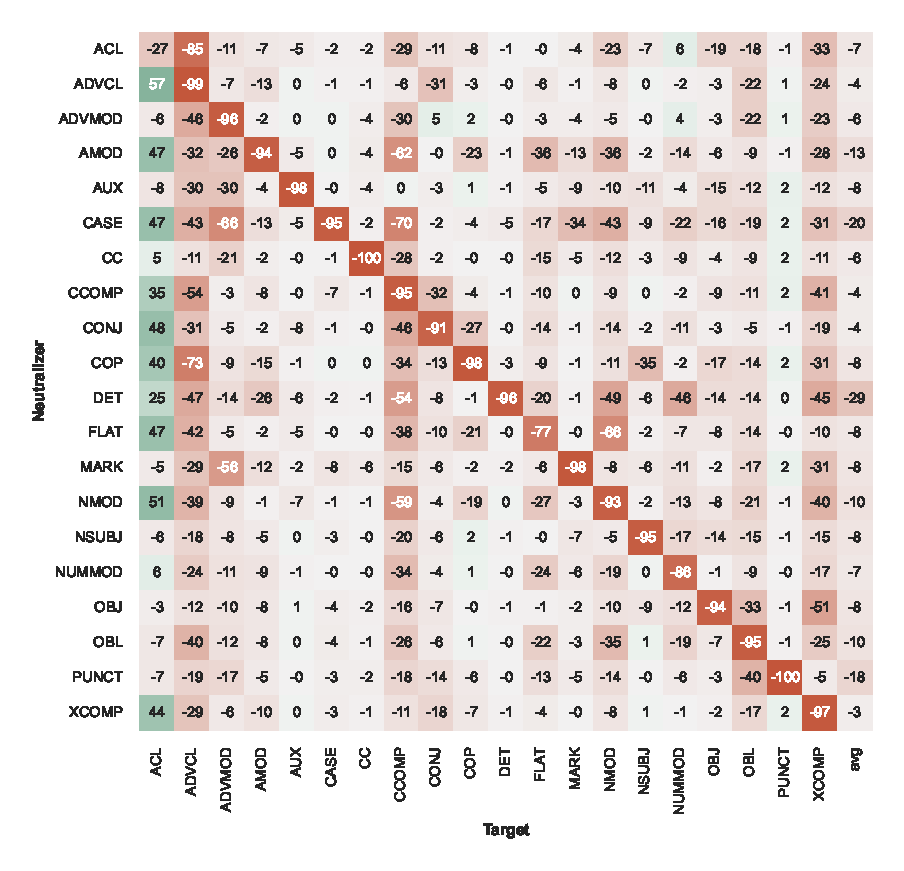
\includegraphics{full_figures/DEP_xlm-roberta-base_el_gdt_acc_drop_agg=mean_probe=9_concat-mode=ONLY.eps}
    \caption{Relative change in accuracy when cross-neutralizing DEP tags using XLM-R embeddings on el\_gdt.}
    \label{fig:xneutr_xlm_dep_gr_complete}
\end{figure*}

% cross-lingual
%% greek
\begin{figure*}[t]
    \centering
    \includegraphics{full_figures/POS-crosslingual-el_gdt_from_en_gum-accdrop.eps}
    \caption{Relative change in accuracy when cross-neutralizing Greek POS tags using English XLM-R embeddings.}
    \label{fig:xlingual_xneutr_pos_el_gdt_from_en_gum}
\end{figure*}

\begin{figure*}[t]
    \centering
    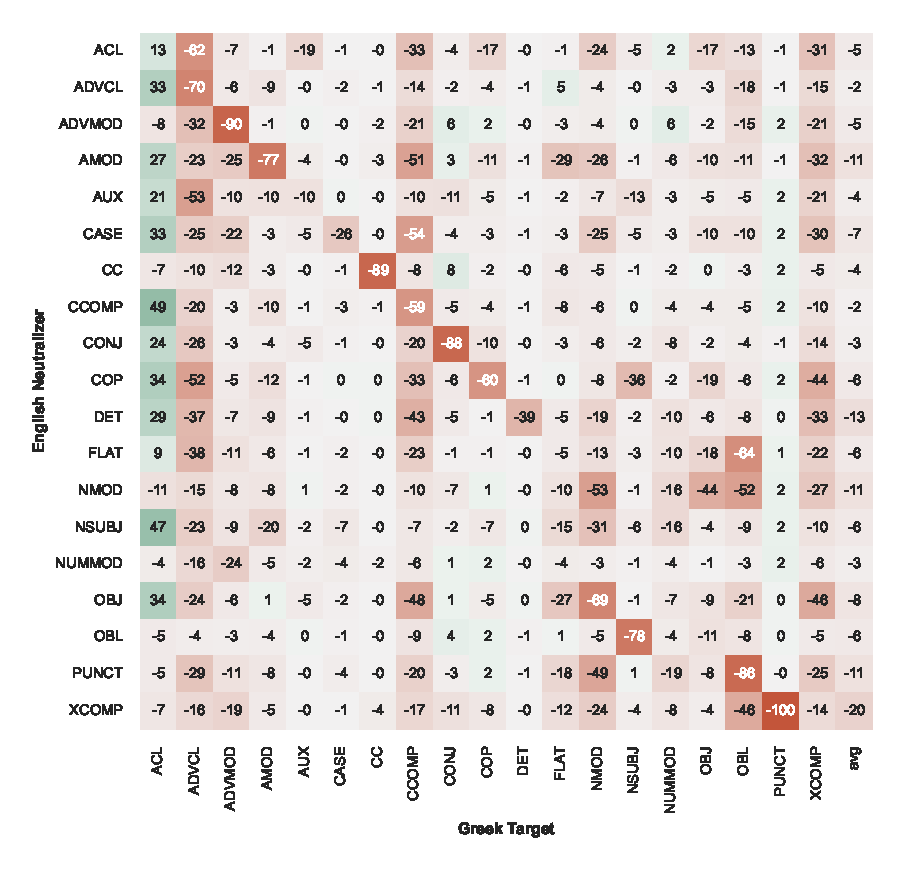
\includegraphics{full_figures/DEP-crosslingual-el_gdt_from_en_gum-accdrop.eps}
    \caption{Relative change in accuracy when cross-neutralizing Greek DEP tags using English XLM-R embeddings.}
    \label{fig:xlingual_xneutr_dep_el_gdt_from_en_gum}
\end{figure*}

\begin{figure*}[t]
    \centering
    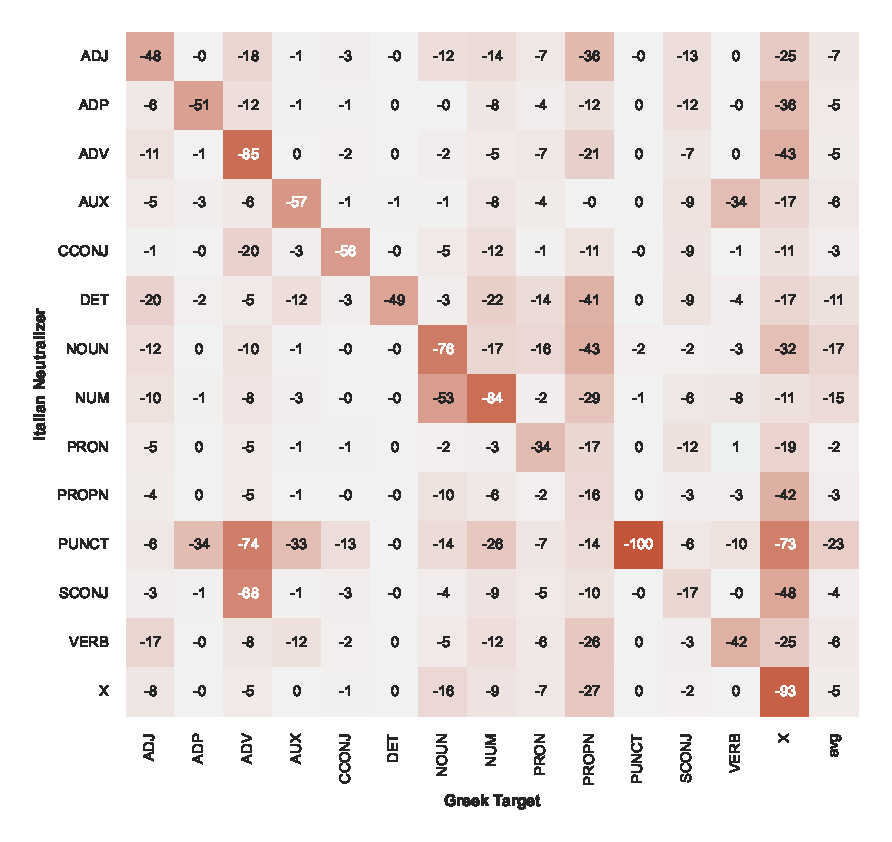
\includegraphics{full_figures/POS-crosslingual-el_gdt_from_it_vit-accdrop.eps}
    \caption{Relative change in accuracy when cross-neutralizing Greek POS tags using Italian XLM-R embeddings.}
    \label{fig:xlingual_xneutr_pos_el_gdt_from_it_vit}
\end{figure*}

\begin{figure*}[t]
    \centering
    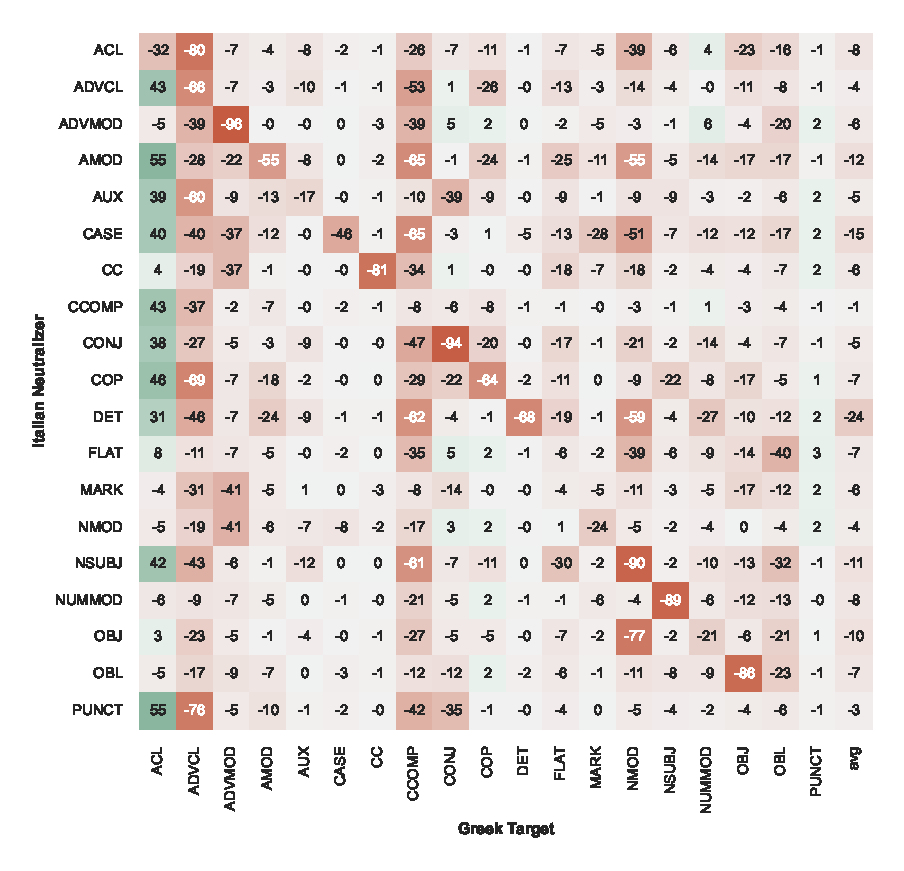
\includegraphics{full_figures/DEP-crosslingual-el_gdt_from_it_vit-accdrop.eps}
    \caption{Relative change in accuracy when cross-neutralizing Greek DEP tags using Italian XLM-R embeddings.}
    \label{fig:xlingual_xneutr_dep_el_gdt_from_it_vit}
\end{figure*}


%% italian
\begin{figure*}[t]
    \centering
    \includegraphics{full_figures/POS-crosslingual-it_vit_from_en_gum-accdrop.eps}
    \caption{Relative change in accuracy when cross-neutralizing Italian POS tags using English XLM-R embeddings.}
    \label{fig:xlingual_xneutr_pos_it_vit_from_en_gum}
\end{figure*}

\begin{figure*}[t]
    \centering
    \includegraphics{full_figures/DEP-crosslingual-it_vit_from_en_gum-accdrop.eps}
    \caption{Relative change in accuracy when cross-neutralizing Italian DEP tags using English XLM-R embeddings.}
    \label{fig:xlingual_xneutr_dep_it_vit_from_en_gum}
\end{figure*}

\begin{figure*}[t]
    \centering
    \includegraphics{full_figures/POS-crosslingual-it_vit_from_el_gdt-accdrop.eps}
    \caption{Relative change in accuracy when cross-neutralizing Italian POS tags using Greek XLM-R embeddings.}
    \label{fig:xlingual_xneutr_pos_it_vit_from_el_gdt}
\end{figure*}

\begin{figure*}[t]
    \centering
    \includegraphics{full_figures/DEP-crosslingual-it_vit_from_el_gdt-accdrop.eps}
    \caption{Relative change in accuracy when cross-neutralizing Italian DEP tags using Greek XLM-R embeddings.}
    \label{fig:xlingual_xneutr_dep_it_vit_from_el_gdt}
\end{figure*}

%% English
\begin{figure*}[t]
    \centering
    \includegraphics{full_figures/POS-crosslingual-en_gum_from_it_vit-accdrop.eps}
    \caption{Relative change in accuracy when cross-neutralizing English POS tags using Italian XLM-R embeddings.}
    \label{fig:xlingual_xneutr_pos_en_gum_from_it_vit}
\end{figure*}

\begin{figure*}[t]
    \centering
    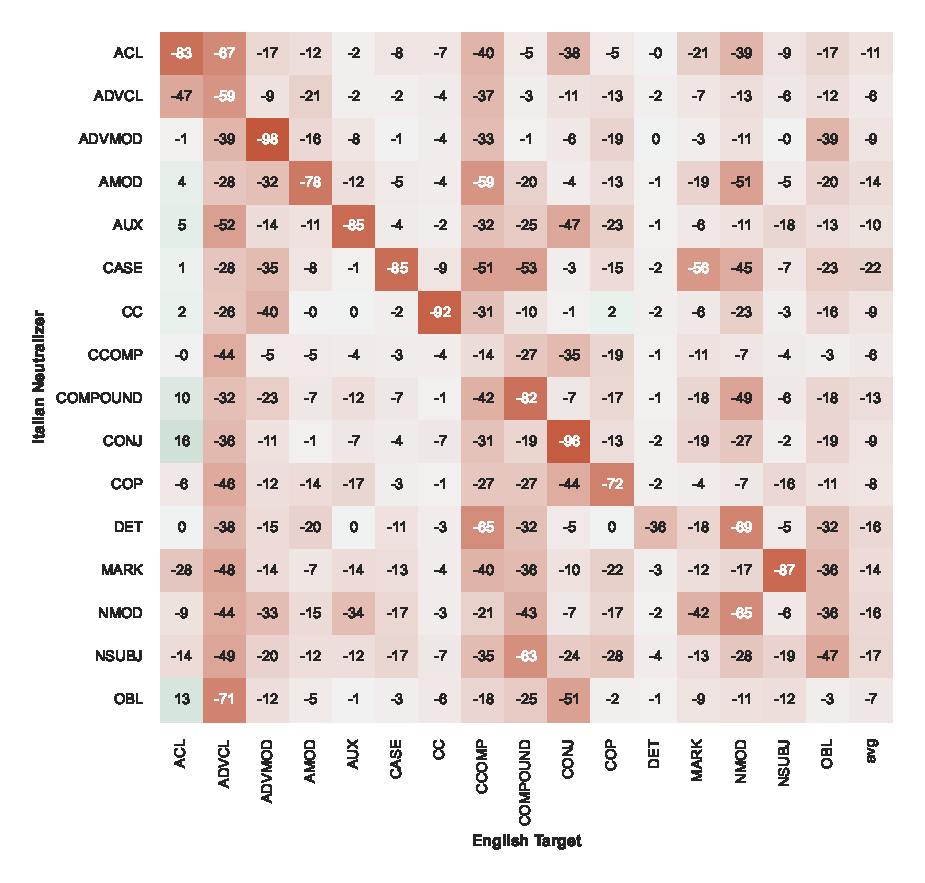
\includegraphics{full_figures/DEP-crosslingual-en_gum_from_it_vit-accdrop.eps}
    \caption{Relative change in accuracy when cross-neutralizing English DEP tags using Italian XLM-R embeddings.}
    \label{fig:xlingual_xneutr_dep_en_gum_from_it_vit}
\end{figure*}

\begin{figure*}[t]
    \centering
    \includegraphics{full_figures/POS-crosslingual-en_gum_from_el_gdt-accdrop.eps}
    \caption{Relative change in accuracy when cross-neutralizing English POS tags using Greek XLM-R embeddings.}
    \label{fig:xlingual_xneutr_pos_en_gum_from_el_gdt}
\end{figure*}

\begin{figure*}[t]
    \centering
    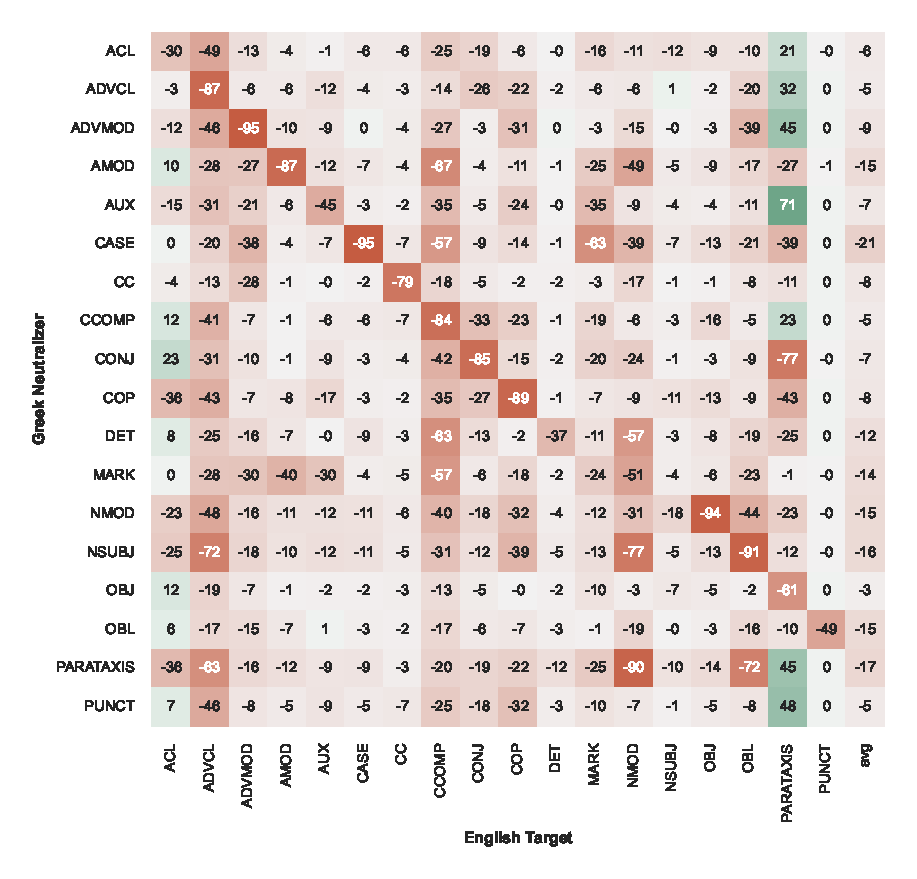
\includegraphics{full_figures/DEP-crosslingual-en_gum_from_el_gdt-accdrop.eps}
    \caption{Relative change in accuracy when cross-neutralizing English DEP tags using Greek XLM-R embeddings.}
    \label{fig:xlingual_xneutr_dep_en_gum_from_el_gdt}
\end{figure*}

\end{document}
